\documentclass[
  bibliography=totoc,     % Literatur im Inhaltsverzeichnis
  captions=tableheading,  % Tabellenüberschriften
  titlepage=firstiscover, % Titelseite ist Deckblatt
]{scrartcl}

% Paket float verbessern
\usepackage{scrhack}

% Warnung, falls nochmal kompiliert werden muss
\usepackage[aux]{rerunfilecheck}

% unverzichtbare Mathe-Befehle
\usepackage{amsmath}
% viele Mathe-Symbole
\usepackage{amssymb}
% Erweiterungen für amsmath
\usepackage{mathtools}

% Fonteinstellungen
\usepackage{fontspec}
% Latin Modern Fonts werden automatisch geladen
% Alternativ zum Beispiel:
%\setromanfont{Libertinus Serif}
%\setsansfont{Libertinus Sans}
%\setmonofont{Libertinus Mono}

% Wenn man andere Schriftarten gesetzt hat,
% sollte man das Seiten-Layout neu berechnen lassen
\recalctypearea{}

% deutsche Spracheinstellungen
\usepackage[ngerman]{babel}


\usepackage[
  math-style=ISO,    % ┐
  bold-style=ISO,    % │
  sans-style=italic, % │ ISO-Standard folgen
  nabla=upright,     % │
  partial=upright,   % │
  mathrm=sym,        % ┘
  warnings-off={           % ┐
    mathtools-colon,       % │ unnötige Warnungen ausschalten
    mathtools-overbracket, % │
  },                       % ┘
]{unicode-math}

% traditionelle Fonts für Mathematik
\setmathfont{Latin Modern Math}
% Alternativ zum Beispiel:
%\setmathfont{Libertinus Math}

\setmathfont{XITS Math}[range={scr, bfscr}]
\setmathfont{XITS Math}[range={cal, bfcal}, StylisticSet=1]

% Zahlen und Einheiten
\usepackage[
  locale=DE,                   % deutsche Einstellungen
  separate-uncertainty=true,   % immer Unsicherheit mit \pm
  per-mode=symbol-or-fraction, % / in inline math, fraction in display math
]{siunitx}

% chemische Formeln
\usepackage[
  version=4,
  math-greek=default, % ┐ mit unicode-math zusammenarbeiten
  text-greek=default, % ┘
]{mhchem}

% richtige Anführungszeichen
\usepackage[autostyle]{csquotes}

% schöne Brüche im Text
\usepackage{xfrac}

% Standardplatzierung für Floats einstellen
\usepackage{float}
\floatplacement{figure}{htbp}
\floatplacement{table}{htbp}

% Floats innerhalb einer Section halten
\usepackage[
  section, % Floats innerhalb der Section halten
  below,   % unterhalb der Section aber auf der selben Seite ist ok
]{placeins}

% Seite drehen für breite Tabellen: landscape Umgebung
\usepackage{pdflscape}

% Captions schöner machen.
\usepackage[
  labelfont=bf,        % Tabelle x: Abbildung y: ist jetzt fett
  font=small,          % Schrift etwas kleiner als Dokument
  width=0.9\textwidth, % maximale Breite einer Caption schmaler
]{caption}
% subfigure, subtable, subref
\usepackage{subcaption}

% Grafiken können eingebunden werden
\usepackage{graphicx}

% schöne Tabellen
\usepackage{tabularray}
\UseTblrLibrary{booktabs, siunitx}

% Verbesserungen am Schriftbild
\usepackage{microtype}

% Literaturverzeichnis
\usepackage[
  backend=biber,
]{biblatex}
% Quellendatenbank
\addbibresource{lit.bib}
\addbibresource{programme.bib}

% Hyperlinks im Dokument
\usepackage[
  german,
  unicode,        % Unicode in PDF-Attributen erlauben
  pdfusetitle,    % Titel, Autoren und Datum als PDF-Attribute
  pdfcreator={},  % ┐ PDF-Attribute säubern
  pdfproducer={}, % ┘
]{hyperref}
% erweiterte Bookmarks im PDF
\usepackage{bookmark}

% Trennung von Wörtern mit Strichen
\usepackage[shortcuts]{extdash}

\author{%
  Vincent Wirsdörfer\\%
  \href{mailto:vincent.wirsdoerfer@udo.edu}{authorA@udo.edu}%
  \and%
  Joris Daus\\%
  \href{mailto:joris.daus@udo.edu}{authorB@udo.edu}%
}
\publishers{TU Dortmund – Fakultät Physik}


\begin{document}
\section{Zielsetzung}
\label{sec:Theorie}

\section{Theorie}

\subsection{Bandstruktur von Festkörpern}

\noindent Eine Möglichkeit um die Struktur von Festkörpern genauer zu beschreiben ist das sogenannte \textit{Bandstrukturmodell}. Betrachtet man das 
freie Elektronengas, so ergibt sich für die Elektronen im Festkörper eine quadratische Dispersionsrelation:

\begin{equation}
    E(k) = \frac{\hbar²{}k²}{2m}
\end{equation}

\noindent Hierbei steht $\hbar$ für das reduzierte Planck'sche Wirkungsquantum, $k$ für die Wellenzahl und $m$ für die Masse des Elektrons.
Wird nun zusätzlich die Anwesenheit eines perioden Gitterpotentials, ausgelöst durch positive Ionenrümpfe, betrachtet, so ergeben sich verbotene
elektronische Zustände. Jene Energieintervalle, dessen Besetzung erlaubt sind werden als \textit{Bänder} bezeichnet. Andere Zustände hingegen, welche
energetisch verboten sind, werden als \textit{Bandlücke} beschrieben. Um einen Eindruck zu gewinnen, wie sich das Bändermodell für spezifische
Elektronenkonfigurationen konkretisiert, ist im Folgenden die Bandstrauktur von Magnesium abgebildet. 

\begin{figure}[H]
    \centering
    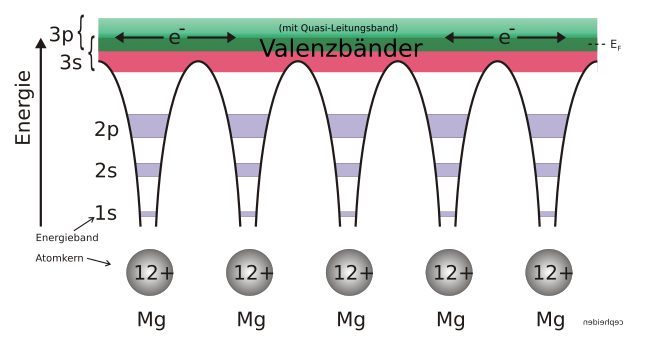
\includegraphics[width=0.7\textwidth]{BandstrukturMagn.png}
    \caption{Bandstruktur von Magnesium.}
    \label{fig:Magnesium}
\end{figure}

\noindent Besonders entscheidend um verschiedene Materialen bzw. Atome zu klassifizieren ist das \textit{Valenz-} und \textit{Leitungsband}. Die Bestzung 
oder Nicht-Besetzung dieser Bänder gibt Aufschluss über die elektrische Leitfähigekit der betrachteten Materialen und wird maßgeblich von der 
\textit{Fermi-Energie} sowie der Größe der \text{Bandlücke} zwischen ihnen beeinflusst. \\

\noindent Bei \textit{Metallen} liegt die Fermi-Energie im Leitungsband und aufgrund der elektronischen Struktur metallischer Stoffe ist der Übergang beider 
Bänder fließend. Die damit verbundene makroskopische Besetzung des Leitungsbandes führt zu einer hohern elektrischen Leitfähigkeit von Metallen.
Im Gegensatz dazu liegt bei \textit{Isolatoren} eine besonders große Bandlücke vor, was die Bestzung des Leitungsbandes ohne starke äußere Anregung verbietet.
Dies erklärt die geringe elektrische Leitfähigekit von Isolatoren. Die Bandstruktur von \textit{Halbleitern} ist grundsätzlich nicht einfach von jener der 
Isolatoren zu unterscheiden. Auch hier liegt die Fermi-Energie unterhalb des Leitungsbandes, jedoch ist die Bandlücke in der Regel geringer, was neue 
Möglichkeiten zur Veränderung elektronischer Eigenschaften bietet. Eine Option ist die sogenannte \textit{Dotierung}, welche jedoch im Späteren 
näher erklärt wird.  

\section{Fehlerrechnung}
\label{sec:Fehlerrechnung}

Alle im Protokoll vermerkten Mittelwerte lassen sich über die folgende Formel berechnen:

\begin{equation}
\label{eqn:Mittelwert}
    \bar{x} = \frac{1}{N}\sum_{i=1}^N x_i
\end{equation}

\noindent Zudem lässt sich der dazugehörige Fehler des Mittelwerts wie folgt berechnen:

\begin{equation}
\label{eqn:Mittelwertfehler}
    \increment \bar{x} = \sqrt{\frac{1}{N\left(N-1\right)}\sum_{i=1}^N \left(x_i - \bar{x}\right)²}
\end{equation}

\noindent Entsteht ein neuer Fehler durch bereits fehlerbehaftete Größen, so wird die Gauß'sche Fehlerfortpflanzung angewendet:

\begin{equation}
\label{eqn:Fehlerfortpflanzung}
    \increment f = \sqrt{\sum_{i=1}^N \left(\frac{\partial f}{\partial x_i}\right)²\cdot\left(\increment x_i\right)²}
\end{equation}

\end{document}